\section{Anatomy of MapReduce Job Execution}
This section introduces the executing procedure of running a MapReduce job in Hadoop.
\begin{figure}[htbp]
%\begin{figure}[!t]
\centering
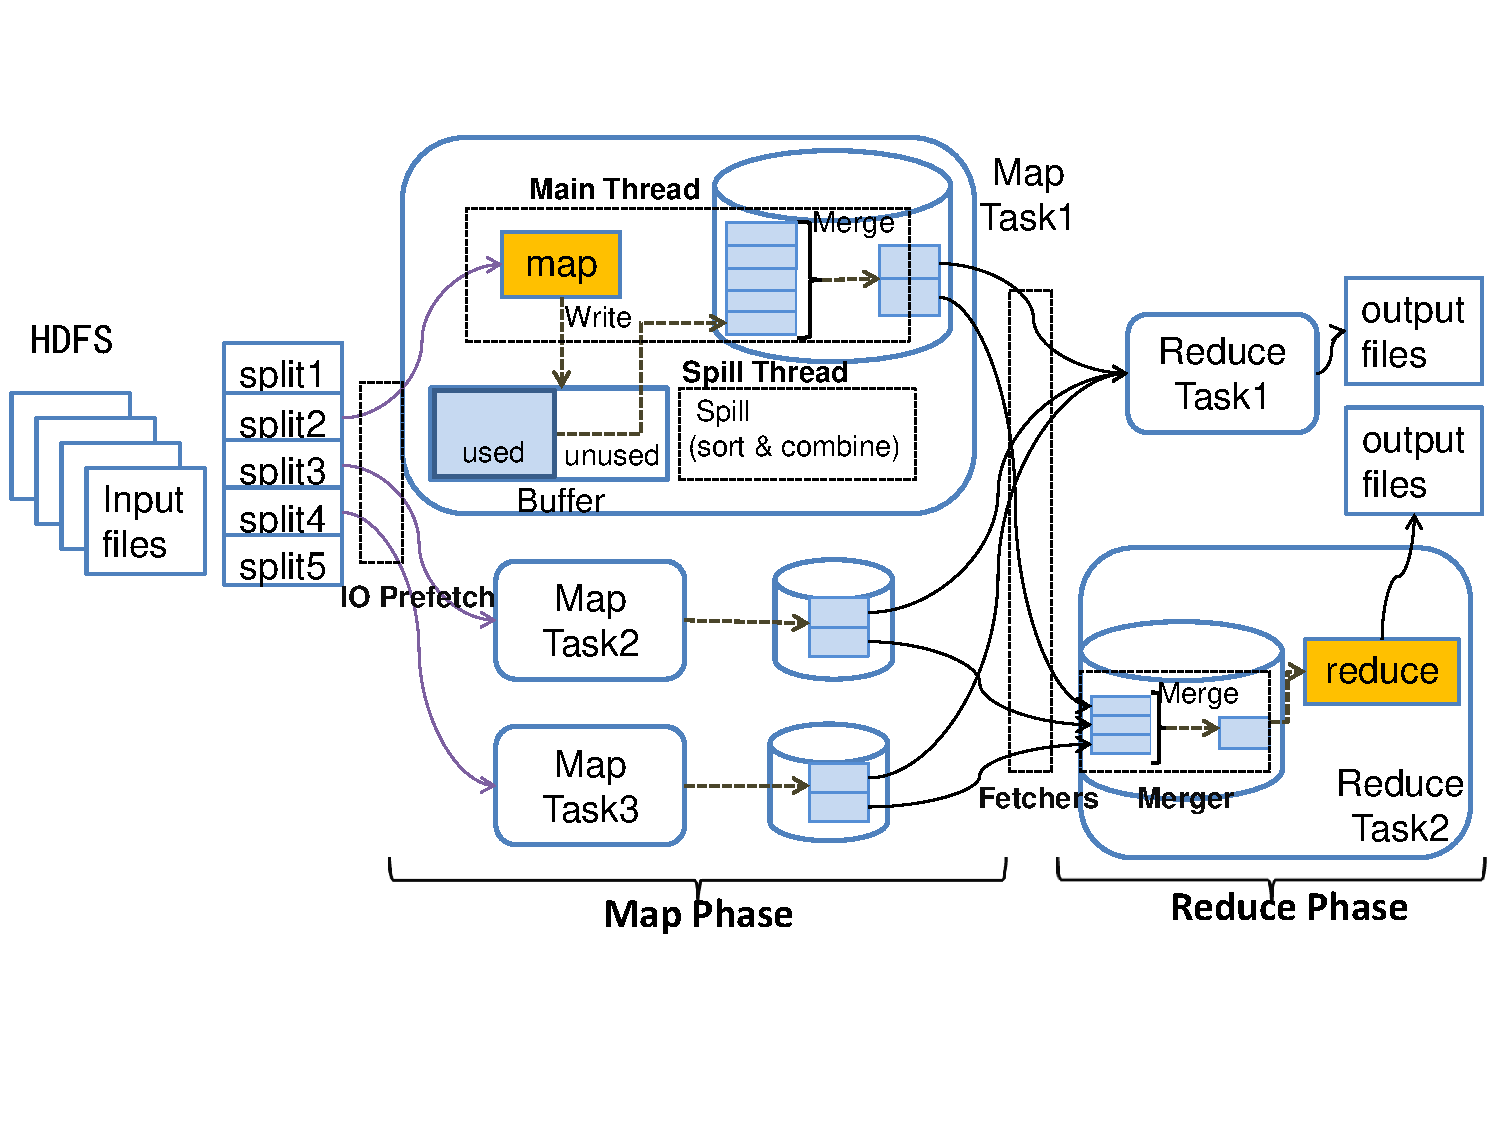
\includegraphics[height=5.25cm, width=8.65cm]{Job}
\caption{The execution procedure of map and reduce tasks}
\label{fig:mrprocedure}
\end{figure}

\noindent\textbf{Map Tasks:}  When the needed resources are allocated to execute a map task, a java process is started on the corresponding node, then the execution environment is initialized. Next the Java process begins to read the input data and run the user-defined Map function. Due to the use of the pre-fetch I/O, the input data to be processed in the map function is read from the input files while the map function is processed. As a consequence, the use of the pre-fetch I/O effectively reduces the cost of reading the data from input files.

As shown in Figure~\ref{fig:mrprocedure}, the execution results of a map function are written into a memory buffer while the size of this buffer is determined by a configuration parameter mapreduce.task.io.mb. A spill thread is started to spill the data of the buffer to the local disks, when the used space of the buffer reaches a pre-configured threshold. As seen above, the procedure of spill consists of two fine-grained phases: \textit{sort} and \textit{combine}. The spill thread first sorts the data of the buffer, then combines and writes the data into a new local disk file. At the beginning of spill, as there is enough buffer space available, the main thread of this java process can still execute the map function and write the output into the buffer until the buffer is full. Therefore, the spill thread, which spills the data of the buffer to the disk, runs in parallel with the main thread to some extent. After the last spill, the main thread merges the outputs of the multiple spills into a new file in some way.

\noindent\textbf{Reduce Tasks:} After some of the map tasks have finished, a new java process is launched to execute reduce tasks. Reduce tasks are initialized first, this java process starts to retrieve data from the output of map tasks. To that end, multiple fetch threads are started to \textit{copy} the outputs of the completed map tasks from remote machines simultaneously, where the number of threads is also a pre-configured parameter. A fetch thread sequentially reads the output of each map task, and the retrieved data is written to the memory or the disk, which is determined by the size of output. In general, the use of multiple fetch threads can accelerate the data shuffle process.

At the same time, a \textit{merge} thread is started to merge the retrieved data either in the memory buffer or on the disk. The merge is run when the used buffer space or the number of disk files reaches the respective pre-configured thresholds. And in this process, the fetch threads and the merge thread normally run in parallel.
%If the fetch thread needs to copy the output of the map task into the buffer, the merge thread is in parallel with the fetch thread when the buffer has enough free space to hold the data. And if the fetch thread should write the output of a map task into the disk file, the merge thread must be in parallel with the fetch thread.
%After the phase of copy, the main thread executes the final merge, which merges the outputs in the memory buffer and on the disk before the execution of the reduce function.
After all the data has been fetched and merged, the reduce function will be executed. Finally, the results of reduce function will be written to HDFS\cite{Shvachko2010The} as the job processing results.
